\documentclass{standalone}
\usepackage{tikz}
\usetikzlibrary{patterns, positioning}
\usepackage[sfdefault]{ClearSans} %% option 'sfdefault' activates Clear Sans as the default text font
\usepackage[T1]{fontenc}

\begin{document}
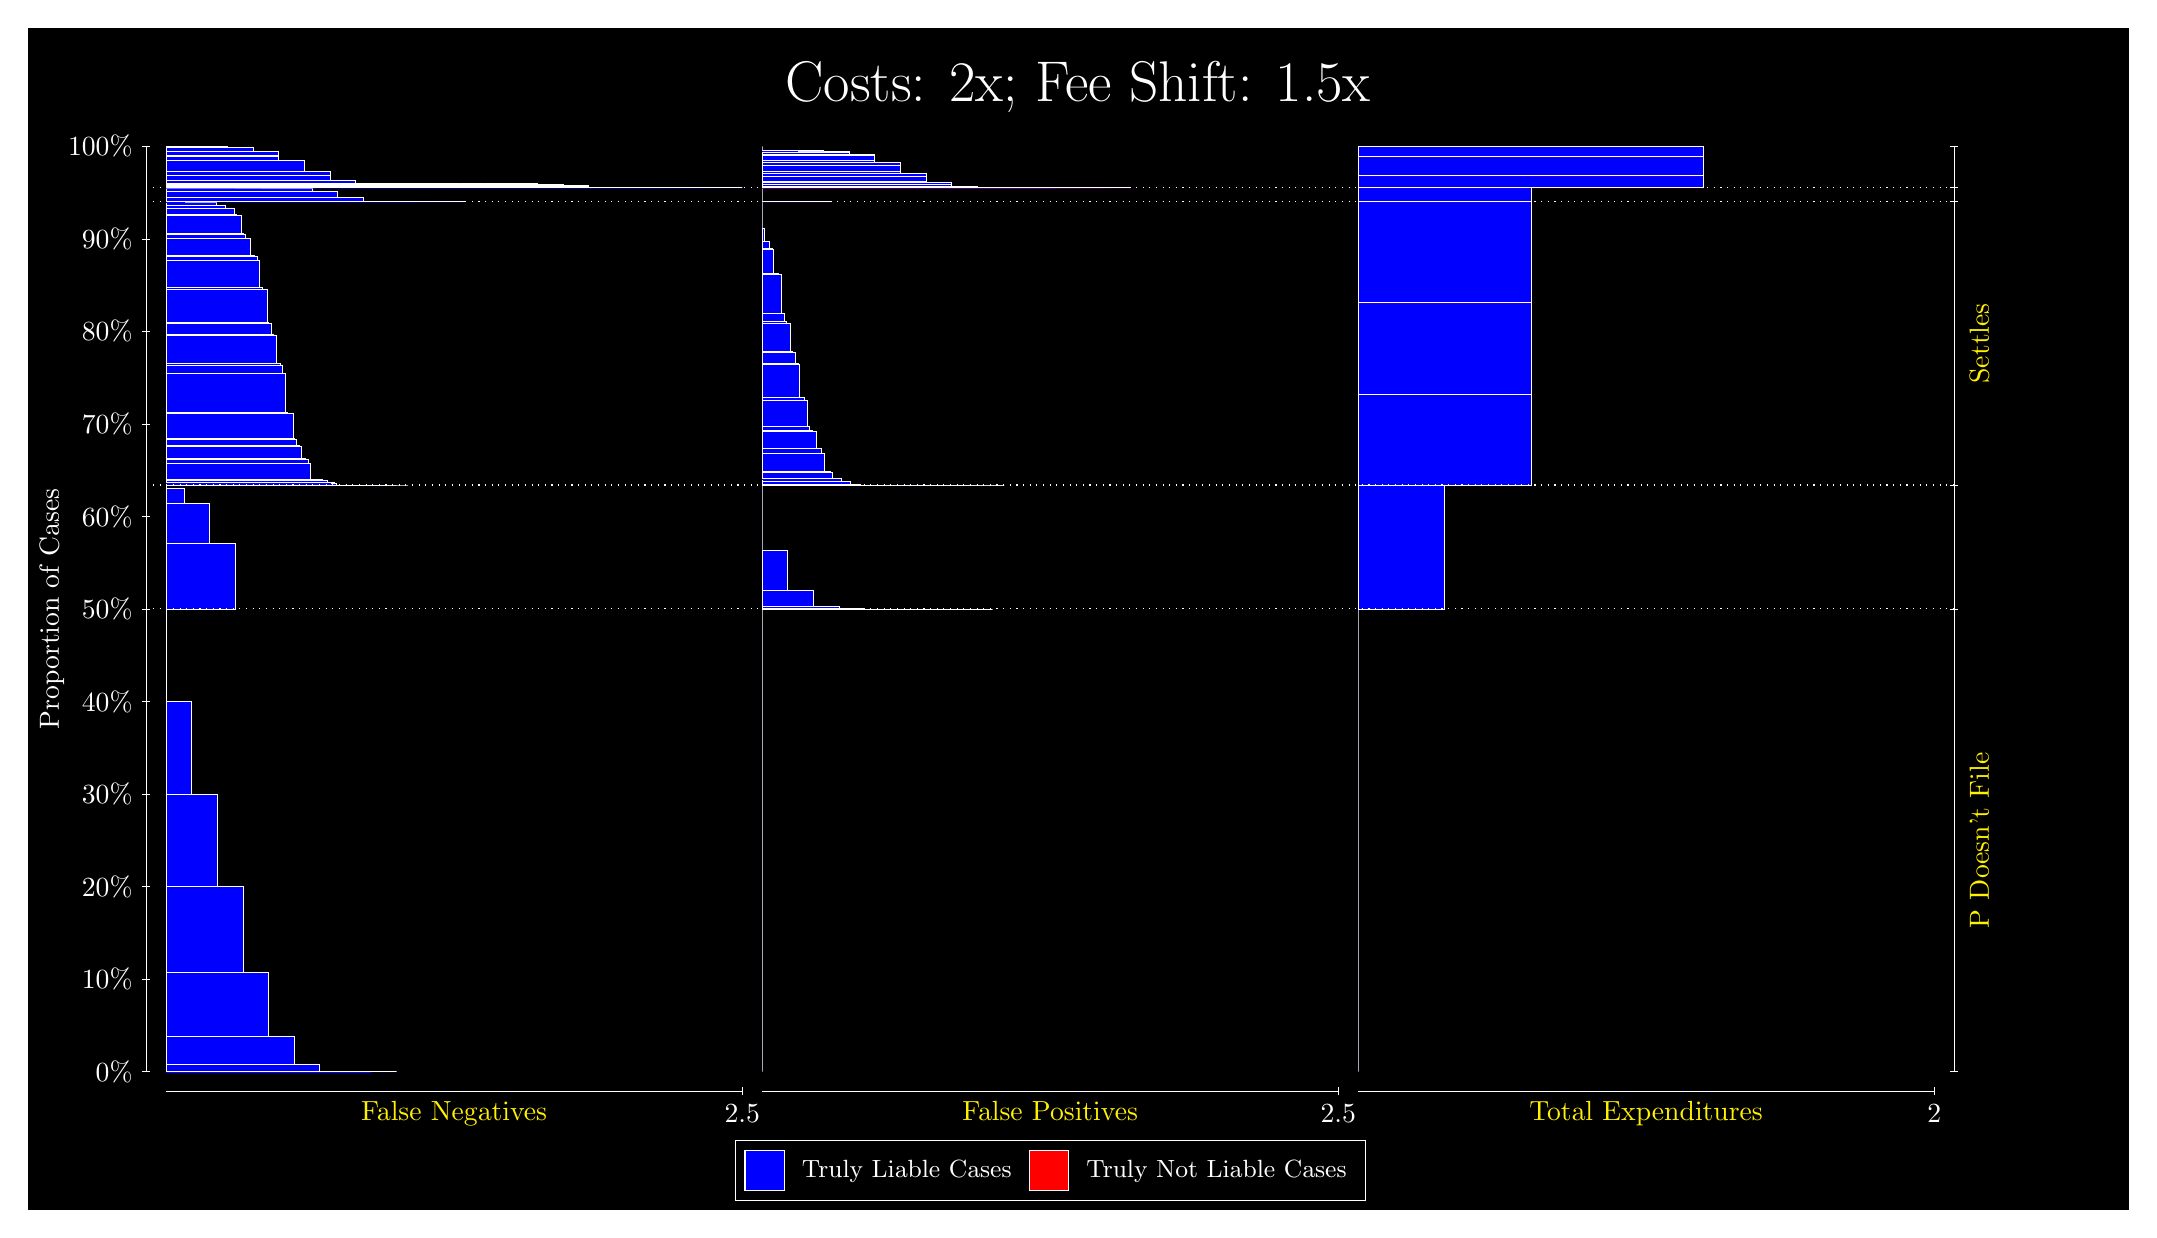
\begin{tikzpicture}
\draw[fill=black] (0,0) rectangle (26.667,15);
\draw[text=white] (0,13.5) rectangle (26.667,15) node[midway] {\huge Costs: 2x; Fee Shift: 1.5x};
\draw[white, very thin] (1.5,1.75) -- (1.5,13.5);
\node[rotate=90, text=white, anchor=center] at (0.3, 7.625) {Proportion of Cases};
\draw[white, very thin] (1.45,1.75) -- (1.55,1.75);
\node[text=white, anchor=east] at (1.45, 1.75) {0\%};
\draw[white, very thin] (1.45,2.925) -- (1.55,2.925);
\node[text=white, anchor=east] at (1.45, 2.925) {10\%};
\draw[white, very thin] (1.45,4.1) -- (1.55,4.1);
\node[text=white, anchor=east] at (1.45, 4.1) {20\%};
\draw[white, very thin] (1.45,5.275) -- (1.55,5.275);
\node[text=white, anchor=east] at (1.45, 5.275) {30\%};
\draw[white, very thin] (1.45,6.45) -- (1.55,6.45);
\node[text=white, anchor=east] at (1.45, 6.45) {40\%};
\draw[white, very thin] (1.45,7.625) -- (1.55,7.625);
\node[text=white, anchor=east] at (1.45, 7.625) {50\%};
\draw[white, very thin] (1.45,8.8) -- (1.55,8.8);
\node[text=white, anchor=east] at (1.45, 8.8) {60\%};
\draw[white, very thin] (1.45,9.975) -- (1.55,9.975);
\node[text=white, anchor=east] at (1.45, 9.975) {70\%};
\draw[white, very thin] (1.45,11.15) -- (1.55,11.15);
\node[text=white, anchor=east] at (1.45, 11.15) {80\%};
\draw[white, very thin] (1.45,12.325) -- (1.55,12.325);
\node[text=white, anchor=east] at (1.45, 12.325) {90\%};
\draw[white, very thin] (1.45,13.5) -- (1.55,13.5);
\node[text=white, anchor=east] at (1.45, 13.5) {100\%};

\draw[white, very thin] (24.457,1.75) -- (24.457,13.5);
\draw[white, very thin] (24.407,1.75) -- (24.507,1.75);
\node[anchor=west] at (24.407, 1.75) {};
\draw[white, very thin] (24.407,7.625) -- (24.507,7.625);
\node[anchor=west] at (24.407, 7.625) {};
\draw[white, very thin] (24.407,9.1989) -- (24.507,9.1989);
\node[anchor=west] at (24.407, 9.1989) {};
\draw[white, very thin] (24.407,12.797) -- (24.507,12.797);
\node[anchor=west] at (24.407, 12.797) {};
\draw[white, very thin] (24.407,12.977) -- (24.507,12.977);
\node[anchor=west] at (24.407, 12.977) {};
\draw[white, very thin] (24.407,13.5) -- (24.507,13.5);
\node[anchor=west] at (24.407, 13.5) {};

\draw[white, very thin, fill=blue] (1.75,1.75) rectangle (4.6775,1.75);
\draw[white, very thin, fill=blue] (1.75,1.75) rectangle (4.3523,1.7503);
\draw[white, very thin, fill=blue] (1.75,1.7503) rectangle (4.027,1.7576);
\draw[white, very thin, fill=blue] (1.75,1.7576) rectangle (3.7017,1.8362);
\draw[white, very thin, fill=blue] (1.75,1.8362) rectangle (3.3764,2.1987);
\draw[white, very thin, fill=blue] (1.75,2.1987) rectangle (3.0511,3.0112);
\draw[white, very thin, fill=blue] (1.75,3.0112) rectangle (2.7258,4.1076);
\draw[white, very thin, fill=blue] (1.75,4.1076) rectangle (2.4006,5.2753);
\draw[white, very thin, fill=blue] (1.75,5.2753) rectangle (2.0753,6.45);
\draw[white, very thin, fill=red] (1.75,6.45) rectangle (1.75,6.45);
\draw[white, very thin, fill=blue] (1.75,6.45) rectangle (1.75,7.625);
\draw[white, very thin, fill=blue] (1.75,7.625) rectangle (2.6283,8.4537);
\draw[white, very thin, fill=blue] (1.75,8.4537) rectangle (2.303,8.967);
\draw[white, very thin, fill=blue] (1.75,8.967) rectangle (1.9777,9.1612);
\draw[white, very thin, fill=red] (1.75,9.1612) rectangle (1.75,9.1612);
\draw[white, very thin, fill=blue] (1.75,9.1612) rectangle (1.75,9.1989);
\draw[white, very thin, fill=blue] (1.75,9.1989) rectangle (4.8239,9.1989);
\draw[white, very thin, fill=blue] (1.75,9.1989) rectangle (4.6775,9.1989);
\draw[white, very thin, fill=blue] (1.75,9.1989) rectangle (4.5312,9.1989);
\draw[white, very thin, fill=blue] (1.75,9.1989) rectangle (4.4986,9.1989);
\draw[white, very thin, fill=blue] (1.75,9.1989) rectangle (4.3848,9.1989);
\draw[white, very thin, fill=blue] (1.75,9.1989) rectangle (4.3523,9.1989);
\draw[white, very thin, fill=blue] (1.75,9.1989) rectangle (4.2384,9.1998);
\draw[white, very thin, fill=blue] (1.75,9.1998) rectangle (4.2059,9.1999);
\draw[white, very thin, fill=blue] (1.75,9.1999) rectangle (4.1734,9.1999);
\draw[white, very thin, fill=blue] (1.75,9.1999) rectangle (4.092,9.2);
\draw[white, very thin, fill=blue] (1.75,9.2) rectangle (4.0595,9.2002);
\draw[white, very thin, fill=blue] (1.75,9.2002) rectangle (4.027,9.2002);
\draw[white, very thin, fill=blue] (1.75,9.2002) rectangle (3.9457,9.2003);
\draw[white, very thin, fill=blue] (1.75,9.2003) rectangle (3.9131,9.2232);
\draw[white, very thin, fill=blue] (1.75,9.2232) rectangle (3.8806,9.229);
\draw[white, very thin, fill=blue] (1.75,9.229) rectangle (3.8481,9.2303);
\draw[white, very thin, fill=blue] (1.75,9.2303) rectangle (3.7993,9.2566);
\draw[white, very thin, fill=blue] (1.75,9.2566) rectangle (3.7668,9.2575);
\draw[white, very thin, fill=blue] (1.75,9.2575) rectangle (3.7342,9.267);
\draw[white, very thin, fill=blue] (1.75,9.267) rectangle (3.7017,9.2691);
\draw[white, very thin, fill=blue] (1.75,9.2691) rectangle (3.6204,9.2707);
\draw[white, very thin, fill=blue] (1.75,9.2707) rectangle (3.5878,9.4749);
\draw[white, very thin, fill=blue] (1.75,9.4749) rectangle (3.5553,9.5266);
\draw[white, very thin, fill=blue] (1.75,9.5266) rectangle (3.5228,9.5391);
\draw[white, very thin, fill=blue] (1.75,9.5391) rectangle (3.474,9.6964);
\draw[white, very thin, fill=blue] (1.75,9.6964) rectangle (3.4415,9.7063);
\draw[white, very thin, fill=blue] (1.75,9.7063) rectangle (3.4089,9.7854);
\draw[white, very thin, fill=blue] (1.75,9.7854) rectangle (3.3764,9.7985);
\draw[white, very thin, fill=blue] (1.75,9.7985) rectangle (3.3602,10.108);
\draw[white, very thin, fill=blue] (1.75,10.108) rectangle (3.2951,10.124);
\draw[white, very thin, fill=blue] (1.75,10.124) rectangle (3.2626,10.616);
\draw[white, very thin, fill=blue] (1.75,10.616) rectangle (3.23,10.721);
\draw[white, very thin, fill=blue] (1.75,10.721) rectangle (3.1975,10.745);
\draw[white, very thin, fill=blue] (1.75,10.745) rectangle (3.1487,11.094);
\draw[white, very thin, fill=blue] (1.75,11.094) rectangle (3.1162,11.115);
\draw[white, very thin, fill=blue] (1.75,11.115) rectangle (3.0837,11.252);
\draw[white, very thin, fill=blue] (1.75,11.252) rectangle (3.0511,11.265);
\draw[white, very thin, fill=blue] (1.75,11.265) rectangle (3.0349,11.683);
\draw[white, very thin, fill=blue] (1.75,11.683) rectangle (2.9698,11.716);
\draw[white, very thin, fill=blue] (1.75,11.716) rectangle (2.9373,12.054);
\draw[white, very thin, fill=blue] (1.75,12.054) rectangle (2.9048,12.107);
\draw[white, very thin, fill=blue] (1.75,12.107) rectangle (2.8722,12.117);
\draw[white, very thin, fill=blue] (1.75,12.117) rectangle (2.8234,12.327);
\draw[white, very thin, fill=blue] (1.75,12.327) rectangle (2.7909,12.335);
\draw[white, very thin, fill=blue] (1.75,12.335) rectangle (2.7584,12.388);
\draw[white, very thin, fill=blue] (1.75,12.388) rectangle (2.7258,12.39);
\draw[white, very thin, fill=blue] (1.75,12.39) rectangle (2.7096,12.626);
\draw[white, very thin, fill=blue] (1.75,12.626) rectangle (2.6445,12.638);
\draw[white, very thin, fill=blue] (1.75,12.638) rectangle (2.612,12.709);
\draw[white, very thin, fill=blue] (1.75,12.709) rectangle (2.5795,12.715);
\draw[white, very thin, fill=blue] (1.75,12.715) rectangle (2.5469,12.715);
\draw[white, very thin, fill=blue] (1.75,12.715) rectangle (2.4982,12.746);
\draw[white, very thin, fill=blue] (1.75,12.746) rectangle (2.4656,12.746);
\draw[white, very thin, fill=blue] (1.75,12.746) rectangle (2.4331,12.751);
\draw[white, very thin, fill=blue] (1.75,12.751) rectangle (2.4006,12.751);
\draw[white, very thin, fill=blue] (1.75,12.751) rectangle (2.3843,12.789);
\draw[white, very thin, fill=blue] (1.75,12.789) rectangle (2.3192,12.79);
\draw[white, very thin, fill=blue] (1.75,12.79) rectangle (2.2867,12.794);
\draw[white, very thin, fill=blue] (1.75,12.794) rectangle (2.2542,12.794);
\draw[white, very thin, fill=blue] (1.75,12.794) rectangle (2.2217,12.794);
\draw[white, very thin, fill=blue] (1.75,12.794) rectangle (2.1729,12.795);
\draw[white, very thin, fill=blue] (1.75,12.795) rectangle (2.1403,12.795);
\draw[white, very thin, fill=blue] (1.75,12.795) rectangle (2.1078,12.795);
\draw[white, very thin, fill=blue] (1.75,12.795) rectangle (2.0753,12.795);
\draw[white, very thin, fill=blue] (1.75,12.795) rectangle (2.059,12.796);
\draw[white, very thin, fill=blue] (1.75,12.796) rectangle (1.994,12.797);
\draw[white, very thin, fill=blue] (1.75,12.797) rectangle (1.9614,12.797);
\draw[white, very thin, fill=blue] (1.75,12.797) rectangle (1.9289,12.797);
\draw[white, very thin, fill=blue] (1.75,12.797) rectangle (1.8964,12.797);
\draw[white, very thin, fill=blue] (1.75,12.797) rectangle (1.8476,12.797);
\draw[white, very thin, fill=blue] (1.75,12.797) rectangle (1.8151,12.797);
\draw[white, very thin, fill=blue] (1.75,12.797) rectangle (1.7825,12.797);
\draw[white, very thin, fill=red] (1.75,12.797) rectangle (1.75,12.797);
\draw[white, very thin, fill=blue] (1.75,12.797) rectangle (1.75,12.797);
\draw[white, very thin, fill=blue] (1.75,12.797) rectangle (5.5558,12.797);
\draw[white, very thin, fill=blue] (1.75,12.797) rectangle (5.2305,12.797);
\draw[white, very thin, fill=blue] (1.75,12.797) rectangle (4.9052,12.797);
\draw[white, very thin, fill=blue] (1.75,12.797) rectangle (4.58,12.802);
\draw[white, very thin, fill=blue] (1.75,12.802) rectangle (4.2547,12.85);
\draw[white, very thin, fill=blue] (1.75,12.85) rectangle (3.9294,12.935);
\draw[white, very thin, fill=blue] (1.75,12.935) rectangle (3.6041,12.972);
\draw[white, very thin, fill=blue] (1.75,12.972) rectangle (3.2788,12.977);
\draw[white, very thin, fill=blue] (1.75,12.977) rectangle (2.9535,12.977);
\draw[white, very thin, fill=blue] (1.75,12.977) rectangle (2.6283,12.977);
\draw[white, very thin, fill=red] (1.75,12.977) rectangle (1.75,12.977);
\draw[white, very thin, fill=blue] (1.75,12.977) rectangle (9.0689,12.977);
\draw[white, very thin, fill=blue] (1.75,12.977) rectangle (8.7436,12.977);
\draw[white, very thin, fill=blue] (1.75,12.977) rectangle (8.4183,12.977);
\draw[white, very thin, fill=blue] (1.75,12.977) rectangle (8.093,12.977);
\draw[white, very thin, fill=blue] (1.75,12.977) rectangle (8.093,12.978);
\draw[white, very thin, fill=blue] (1.75,12.978) rectangle (7.7677,12.978);
\draw[white, very thin, fill=blue] (1.75,12.978) rectangle (7.4425,12.979);
\draw[white, very thin, fill=blue] (1.75,12.979) rectangle (7.4425,12.981);
\draw[white, very thin, fill=blue] (1.75,12.981) rectangle (7.4425,12.982);
\draw[white, very thin, fill=blue] (1.75,12.982) rectangle (7.1172,12.992);
\draw[white, very thin, fill=blue] (1.75,12.992) rectangle (7.1172,12.999);
\draw[white, very thin, fill=blue] (1.75,12.999) rectangle (6.7919,13.015);
\draw[white, very thin, fill=blue] (1.75,13.015) rectangle (6.7919,13.023);
\draw[white, very thin, fill=blue] (1.75,13.023) rectangle (6.4666,13.029);
\draw[white, very thin, fill=blue] (1.75,13.029) rectangle (6.4666,13.031);
\draw[white, very thin, fill=blue] (1.75,13.031) rectangle (6.1413,13.032);
\draw[white, very thin, fill=blue] (1.75,13.032) rectangle (5.816,13.032);
\draw[white, very thin, fill=blue] (1.75,13.032) rectangle (5.7835,13.032);
\draw[white, very thin, fill=blue] (1.75,13.032) rectangle (5.4908,13.032);
\draw[white, very thin, fill=blue] (1.75,13.032) rectangle (5.4908,13.032);
\draw[white, very thin, fill=blue] (1.75,13.032) rectangle (5.4582,13.032);
\draw[white, very thin, fill=blue] (1.75,13.032) rectangle (5.1655,13.032);
\draw[white, very thin, fill=blue] (1.75,13.032) rectangle (5.1329,13.032);
\draw[white, very thin, fill=blue] (1.75,13.032) rectangle (4.8402,13.032);
\draw[white, very thin, fill=blue] (1.75,13.032) rectangle (4.8077,13.032);
\draw[white, very thin, fill=blue] (1.75,13.032) rectangle (4.8077,13.032);
\draw[white, very thin, fill=blue] (1.75,13.032) rectangle (4.4824,13.034);
\draw[white, very thin, fill=blue] (1.75,13.034) rectangle (4.4824,13.036);
\draw[white, very thin, fill=blue] (1.75,13.036) rectangle (4.1571,13.073);
\draw[white, very thin, fill=blue] (1.75,13.073) rectangle (3.8318,13.127);
\draw[white, very thin, fill=blue] (1.75,13.127) rectangle (3.8318,13.18);
\draw[white, very thin, fill=blue] (1.75,13.18) rectangle (3.5065,13.323);
\draw[white, very thin, fill=blue] (1.75,13.323) rectangle (3.1812,13.377);
\draw[white, very thin, fill=blue] (1.75,13.377) rectangle (3.1812,13.38);
\draw[white, very thin, fill=blue] (1.75,13.38) rectangle (3.1812,13.435);
\draw[white, very thin, fill=blue] (1.75,13.435) rectangle (2.856,13.485);
\draw[white, very thin, fill=blue] (1.75,13.485) rectangle (2.856,13.487);
\draw[white, very thin, fill=blue] (1.75,13.487) rectangle (2.5307,13.491);
\draw[white, very thin, fill=blue] (1.75,13.491) rectangle (2.5307,13.491);
\draw[white, very thin, fill=blue] (1.75,13.491) rectangle (2.5307,13.498);
\draw[white, very thin, fill=blue] (1.75,13.498) rectangle (2.2054,13.5);
\draw[white, very thin, fill=blue] (1.75,13.5) rectangle (2.2054,13.5);
\draw[white, very thin, fill=blue] (1.75,13.5) rectangle (1.8801,13.5);
\draw[white, very thin, fill=blue] (1.75,13.5) rectangle (1.8801,13.5);
\draw[white, very thin, fill=red] (1.75,13.5) rectangle (1.75,13.5);
\draw[white, very thin, fill=blue] (1.75,13.5) rectangle (1.75,13.5);
\draw[white, very thin, fill=red] (9.3189,1.75) rectangle (9.3189,1.75);
\draw[white, very thin, fill=blue] (9.3189,1.75) rectangle (9.3189,7.625);
\draw[white, very thin, fill=red] (9.3189,7.625) rectangle (12.246,7.625);
\draw[white, very thin, fill=blue] (9.3189,7.625) rectangle (12.246,7.625);
\draw[white, very thin, fill=blue] (9.3189,7.625) rectangle (11.921,7.625);
\draw[white, very thin, fill=blue] (9.3189,7.625) rectangle (11.596,7.625);
\draw[white, very thin, fill=blue] (9.3189,7.625) rectangle (11.271,7.625);
\draw[white, very thin, fill=blue] (9.3189,7.625) rectangle (10.945,7.625);
\draw[white, very thin, fill=blue] (9.3189,7.625) rectangle (10.62,7.6273);
\draw[white, very thin, fill=blue] (9.3189,7.6273) rectangle (10.295,7.6627);
\draw[white, very thin, fill=blue] (9.3189,7.6627) rectangle (9.9694,7.857);
\draw[white, very thin, fill=blue] (9.3189,7.857) rectangle (9.6442,8.3702);
\draw[white, very thin, fill=blue] (9.3189,8.3702) rectangle (9.3189,9.1989);
\draw[white, very thin, fill=red] (9.3189,9.1989) rectangle (12.393,9.1989);
\draw[white, very thin, fill=blue] (9.3189,9.1989) rectangle (12.393,9.1989);
\draw[white, very thin, fill=blue] (9.3189,9.1989) rectangle (12.068,9.1989);
\draw[white, very thin, fill=red] (9.3189,9.1989) rectangle (11.954,9.1989);
\draw[white, very thin, fill=blue] (9.3189,9.1989) rectangle (11.954,9.1989);
\draw[white, very thin, fill=red] (9.3189,9.1989) rectangle (11.807,9.1989);
\draw[white, very thin, fill=blue] (9.3189,9.1989) rectangle (11.807,9.1989);
\draw[white, very thin, fill=blue] (9.3189,9.1989) rectangle (11.742,9.1989);
\draw[white, very thin, fill=red] (9.3189,9.1989) rectangle (11.661,9.1989);
\draw[white, very thin, fill=blue] (9.3189,9.1989) rectangle (11.661,9.1989);
\draw[white, very thin, fill=blue] (9.3189,9.1989) rectangle (11.628,9.1989);
\draw[white, very thin, fill=red] (9.3189,9.1989) rectangle (11.515,9.1989);
\draw[white, very thin, fill=blue] (9.3189,9.1989) rectangle (11.515,9.1989);
\draw[white, very thin, fill=blue] (9.3189,9.1989) rectangle (11.482,9.1989);
\draw[white, very thin, fill=blue] (9.3189,9.1989) rectangle (11.417,9.1989);
\draw[white, very thin, fill=red] (9.3189,9.1989) rectangle (11.368,9.1989);
\draw[white, very thin, fill=blue] (9.3189,9.1989) rectangle (11.368,9.1989);
\draw[white, very thin, fill=blue] (9.3189,9.1989) rectangle (11.336,9.1989);
\draw[white, very thin, fill=blue] (9.3189,9.1989) rectangle (11.303,9.1989);
\draw[white, very thin, fill=red] (9.3189,9.1989) rectangle (11.222,9.1989);
\draw[white, very thin, fill=blue] (9.3189,9.1989) rectangle (11.222,9.1989);
\draw[white, very thin, fill=blue] (9.3189,9.1989) rectangle (11.189,9.1989);
\draw[white, very thin, fill=blue] (9.3189,9.1989) rectangle (11.157,9.1989);
\draw[white, very thin, fill=blue] (9.3189,9.1989) rectangle (11.092,9.1989);
\draw[white, very thin, fill=red] (9.3189,9.1989) rectangle (11.075,9.1989);
\draw[white, very thin, fill=blue] (9.3189,9.1989) rectangle (11.075,9.1989);
\draw[white, very thin, fill=blue] (9.3189,9.1989) rectangle (11.043,9.1989);
\draw[white, very thin, fill=blue] (9.3189,9.1989) rectangle (11.01,9.1989);
\draw[white, very thin, fill=blue] (9.3189,9.1989) rectangle (10.978,9.1989);
\draw[white, very thin, fill=red] (9.3189,9.1989) rectangle (10.929,9.1989);
\draw[white, very thin, fill=blue] (9.3189,9.1989) rectangle (10.929,9.1989);
\draw[white, very thin, fill=blue] (9.3189,9.1989) rectangle (10.896,9.1989);
\draw[white, very thin, fill=blue] (9.3189,9.1989) rectangle (10.864,9.199);
\draw[white, very thin, fill=blue] (9.3189,9.199) rectangle (10.831,9.199);
\draw[white, very thin, fill=blue] (9.3189,9.199) rectangle (10.766,9.2004);
\draw[white, very thin, fill=blue] (9.3189,9.2004) rectangle (10.75,9.2004);
\draw[white, very thin, fill=blue] (9.3189,9.2004) rectangle (10.718,9.2005);
\draw[white, very thin, fill=blue] (9.3189,9.2005) rectangle (10.685,9.2005);
\draw[white, very thin, fill=blue] (9.3189,9.2005) rectangle (10.653,9.2015);
\draw[white, very thin, fill=blue] (9.3189,9.2015) rectangle (10.604,9.2015);
\draw[white, very thin, fill=blue] (9.3189,9.2015) rectangle (10.571,9.2017);
\draw[white, very thin, fill=blue] (9.3189,9.2017) rectangle (10.539,9.2059);
\draw[white, very thin, fill=blue] (9.3189,9.2059) rectangle (10.506,9.2067);
\draw[white, very thin, fill=blue] (9.3189,9.2067) rectangle (10.441,9.2445);
\draw[white, very thin, fill=blue] (9.3189,9.2445) rectangle (10.425,9.2445);
\draw[white, very thin, fill=blue] (9.3189,9.2445) rectangle (10.392,9.2491);
\draw[white, very thin, fill=blue] (9.3189,9.2491) rectangle (10.36,9.2495);
\draw[white, very thin, fill=blue] (9.3189,9.2495) rectangle (10.327,9.2801);
\draw[white, very thin, fill=blue] (9.3189,9.2801) rectangle (10.278,9.2808);
\draw[white, very thin, fill=blue] (9.3189,9.2808) rectangle (10.246,9.287);
\draw[white, very thin, fill=blue] (9.3189,9.287) rectangle (10.213,9.3574);
\draw[white, very thin, fill=blue] (9.3189,9.3574) rectangle (10.181,9.3698);
\draw[white, very thin, fill=blue] (9.3189,9.3698) rectangle (10.116,9.6057);
\draw[white, very thin, fill=blue] (9.3189,9.6057) rectangle (10.1,9.6078);
\draw[white, very thin, fill=blue] (9.3189,9.6078) rectangle (10.067,9.6606);
\draw[white, very thin, fill=blue] (9.3189,9.6606) rectangle (10.034,9.6682);
\draw[white, very thin, fill=blue] (9.3189,9.6682) rectangle (10.002,9.8786);
\draw[white, very thin, fill=blue] (9.3189,9.8786) rectangle (9.9532,9.8881);
\draw[white, very thin, fill=blue] (9.3189,9.8881) rectangle (9.9206,9.9418);
\draw[white, very thin, fill=blue] (9.3189,9.9418) rectangle (9.8881,10.279);
\draw[white, very thin, fill=blue] (9.3189,10.279) rectangle (9.8556,10.313);
\draw[white, very thin, fill=blue] (9.3189,10.313) rectangle (9.7905,10.73);
\draw[white, very thin, fill=blue] (9.3189,10.73) rectangle (9.7743,10.743);
\draw[white, very thin, fill=blue] (9.3189,10.743) rectangle (9.7417,10.88);
\draw[white, very thin, fill=blue] (9.3189,10.88) rectangle (9.7092,10.901);
\draw[white, very thin, fill=blue] (9.3189,10.901) rectangle (9.6767,11.25);
\draw[white, very thin, fill=blue] (9.3189,11.25) rectangle (9.6279,11.275);
\draw[white, very thin, fill=blue] (9.3189,11.275) rectangle (9.5954,11.38);
\draw[white, very thin, fill=blue] (9.3189,11.38) rectangle (9.5628,11.872);
\draw[white, very thin, fill=blue] (9.3189,11.872) rectangle (9.5303,11.888);
\draw[white, very thin, fill=blue] (9.3189,11.888) rectangle (9.4652,12.197);
\draw[white, very thin, fill=blue] (9.3189,12.197) rectangle (9.449,12.21);
\draw[white, very thin, fill=blue] (9.3189,12.21) rectangle (9.4165,12.289);
\draw[white, very thin, fill=blue] (9.3189,12.289) rectangle (9.3839,12.299);
\draw[white, very thin, fill=blue] (9.3189,12.299) rectangle (9.3514,12.456);
\draw[white, very thin, fill=blue] (9.3189,12.456) rectangle (9.3189,12.797);
\draw[white, very thin, fill=red] (9.3189,12.797) rectangle (10.197,12.797);
\draw[white, very thin, fill=blue] (9.3189,12.797) rectangle (10.197,12.797);
\draw[white, very thin, fill=blue] (9.3189,12.797) rectangle (9.8718,12.797);
\draw[white, very thin, fill=blue] (9.3189,12.797) rectangle (9.5466,12.802);
\draw[white, very thin, fill=blue] (9.3189,12.802) rectangle (9.3189,12.977);
\draw[white, very thin, fill=red] (9.3189,12.977) rectangle (14.003,12.977);
\draw[white, very thin, fill=blue] (9.3189,12.977) rectangle (14.003,12.977);
\draw[white, very thin, fill=red] (9.3189,12.977) rectangle (13.678,12.977);
\draw[white, very thin, fill=blue] (9.3189,12.977) rectangle (13.678,12.977);
\draw[white, very thin, fill=red] (9.3189,12.977) rectangle (13.352,12.977);
\draw[white, very thin, fill=blue] (9.3189,12.977) rectangle (13.352,12.977);
\draw[white, very thin, fill=blue] (9.3189,12.977) rectangle (13.027,12.977);
\draw[white, very thin, fill=red] (9.3189,12.977) rectangle (13.027,12.977);
\draw[white, very thin, fill=blue] (9.3189,12.977) rectangle (13.027,12.977);
\draw[white, very thin, fill=blue] (9.3189,12.977) rectangle (12.702,12.978);
\draw[white, very thin, fill=red] (9.3189,12.978) rectangle (12.702,12.978);
\draw[white, very thin, fill=blue] (9.3189,12.978) rectangle (12.702,12.978);
\draw[white, very thin, fill=blue] (9.3189,12.978) rectangle (12.377,12.979);
\draw[white, very thin, fill=red] (9.3189,12.979) rectangle (12.377,12.979);
\draw[white, very thin, fill=blue] (9.3189,12.979) rectangle (12.377,12.979);
\draw[white, very thin, fill=blue] (9.3189,12.979) rectangle (12.051,12.984);
\draw[white, very thin, fill=red] (9.3189,12.984) rectangle (12.051,12.984);
\draw[white, very thin, fill=blue] (9.3189,12.984) rectangle (12.051,12.991);
\draw[white, very thin, fill=blue] (9.3189,12.991) rectangle (12.051,12.991);
\draw[white, very thin, fill=blue] (9.3189,12.991) rectangle (12.051,12.991);
\draw[white, very thin, fill=blue] (9.3189,12.991) rectangle (11.726,13.022);
\draw[white, very thin, fill=red] (9.3189,13.022) rectangle (11.726,13.022);
\draw[white, very thin, fill=blue] (9.3189,13.022) rectangle (11.726,13.042);
\draw[white, very thin, fill=blue] (9.3189,13.042) rectangle (11.726,13.042);
\draw[white, very thin, fill=blue] (9.3189,13.042) rectangle (11.401,13.057);
\draw[white, very thin, fill=blue] (9.3189,13.057) rectangle (11.401,13.116);
\draw[white, very thin, fill=blue] (9.3189,13.116) rectangle (11.401,13.154);
\draw[white, very thin, fill=blue] (9.3189,13.154) rectangle (11.075,13.181);
\draw[white, very thin, fill=blue] (9.3189,13.181) rectangle (11.075,13.254);
\draw[white, very thin, fill=blue] (9.3189,13.254) rectangle (11.075,13.297);
\draw[white, very thin, fill=blue] (9.3189,13.297) rectangle (10.75,13.325);
\draw[white, very thin, fill=blue] (9.3189,13.325) rectangle (10.75,13.326);
\draw[white, very thin, fill=blue] (9.3189,13.326) rectangle (10.75,13.385);
\draw[white, very thin, fill=blue] (9.3189,13.385) rectangle (10.75,13.404);
\draw[white, very thin, fill=blue] (9.3189,13.404) rectangle (10.425,13.42);
\draw[white, very thin, fill=blue] (9.3189,13.42) rectangle (10.425,13.441);
\draw[white, very thin, fill=blue] (9.3189,13.441) rectangle (10.1,13.442);
\draw[white, very thin, fill=blue] (9.3189,13.442) rectangle (10.1,13.445);
\draw[white, very thin, fill=blue] (9.3189,13.445) rectangle (10.1,13.445);
\draw[white, very thin, fill=blue] (9.3189,13.445) rectangle (9.7743,13.445);
\draw[white, very thin, fill=blue] (9.3189,13.445) rectangle (9.7743,13.446);
\draw[white, very thin, fill=red] (9.3189,13.446) rectangle (9.7417,13.446);
\draw[white, very thin, fill=blue] (9.3189,13.446) rectangle (9.7417,13.446);
\draw[white, very thin, fill=blue] (9.3189,13.446) rectangle (9.449,13.446);
\draw[white, very thin, fill=blue] (9.3189,13.446) rectangle (9.449,13.446);
\draw[white, very thin, fill=blue] (9.3189,13.446) rectangle (9.449,13.446);
\draw[white, very thin, fill=red] (9.3189,13.446) rectangle (9.4165,13.446);
\draw[white, very thin, fill=blue] (9.3189,13.446) rectangle (9.4165,13.446);
\draw[white, very thin, fill=red] (9.3189,13.446) rectangle (9.3189,13.446);
\draw[white, very thin, fill=blue] (9.3189,13.446) rectangle (9.3189,13.5);
\draw[white, very thin, fill=red] (16.888,1.75) rectangle (16.888,1.75);
\draw[white, very thin, fill=blue] (16.888,1.75) rectangle (16.888,7.625);
\draw[white, very thin, fill=red] (16.888,7.625) rectangle (17.986,7.625);
\draw[white, very thin, fill=blue] (16.888,7.625) rectangle (17.986,9.1989);
\draw[white, very thin, fill=red] (16.888,9.1989) rectangle (19.083,9.1989);
\draw[white, very thin, fill=blue] (16.888,9.1989) rectangle (19.083,10.354);
\draw[white, very thin, fill=red] (16.888,10.354) rectangle (19.083,10.354);
\draw[white, very thin, fill=blue] (16.888,10.354) rectangle (19.083,11.516);
\draw[white, very thin, fill=red] (16.888,11.516) rectangle (19.083,11.516);
\draw[white, very thin, fill=blue] (16.888,11.516) rectangle (19.083,12.797);
\draw[white, very thin, fill=red] (16.888,12.797) rectangle (19.083,12.797);
\draw[white, very thin, fill=blue] (16.888,12.797) rectangle (19.083,12.977);
\draw[white, very thin, fill=red] (16.888,12.977) rectangle (21.279,12.977);
\draw[white, very thin, fill=blue] (16.888,12.977) rectangle (21.279,13.128);
\draw[white, very thin, fill=red] (16.888,13.128) rectangle (21.279,13.128);
\draw[white, very thin, fill=blue] (16.888,13.128) rectangle (21.279,13.369);
\draw[white, very thin, fill=red] (16.888,13.369) rectangle (21.279,13.369);
\draw[white, very thin, fill=blue] (16.888,13.369) rectangle (21.279,13.5);
\draw[white, dotted] (1.5,7.625) -- (24.457,7.625);
\draw[white, dotted] (1.5,9.1989) -- (24.457,9.1989);
\draw[white, dotted] (1.5,12.797) -- (24.457,12.797);
\draw[white, dotted] (1.5,12.977) -- (24.457,12.977);
\draw[white, very thin] (1.75,1.5) -- (9.0689,1.5);
\node[text=yellow, anchor=north] at (5.4094, 1.5) {False Negatives};
\draw[white, very thin] (9.0689,1.45) -- (9.0689,1.55);
\node[text=white, anchor=north] at (9.0689, 1.45) {2.5};

\draw[white, very thin] (9.3189,1.5) -- (16.638,1.5);
\node[text=yellow, anchor=north] at (12.978, 1.5) {False Positives};
\draw[white, very thin] (16.638,1.45) -- (16.638,1.55);
\node[text=white, anchor=north] at (16.638, 1.45) {2.5};

\draw[white, very thin] (16.888,1.5) -- (24.207,1.5);
\node[text=yellow, anchor=north] at (20.547, 1.5) {Total Expenditures};
\draw[white, very thin] (24.207,1.45) -- (24.207,1.55);
\node[text=white, anchor=north] at (24.207, 1.45) {2};

\node[text=yellow, centered, rotate=90] at (24.777, 4.6875) {P Doesn't File};

\node[text=yellow, centered, rotate=90] at (24.777, 10.998) {Settles};



\draw (12.978300999999998,1.5) node[draw=none] (baseCoordinate) {};
\begin{scope}[align=center]
        \matrix[scale=0.5, draw=white, below=0.5cm of baseCoordinate, nodes={draw}, column sep=0.1cm]{
            \node[rectangle, draw, minimum width=0.5cm, minimum height=0.5cm, fill=blue] {}; &
            \node[draw=none, font=\small, text=white] (B) {Truly Liable Cases}; &
            \node[rectangle, draw, minimum width=0.5cm, minimum height=0.5cm, fill=red] {}; &
            \node[draw=none, font=\small, text=white] (B) {Truly Not Liable Cases}; \\
            };
\end{scope}

\end{tikzpicture}
\end{document}